%%%%%%%%%%%%%%%%%%%%%%%%%%%%%%%%%%%%%%%%%%%%%%%%%%%%%%%%%%%%%%%%%%%%%%%%%%%
\subsubsection{\label{sec:Globus-Protocols}Globus Protocols and Terminology}
%%%%%%%%%%%%%%%%%%%%%%%%%%%%%%%%%%%%%%%%%%%%%%%%%%%%%%%%%%%%%%%%%%%%%%%%%%%
The Globus software provides a well-defined set of protocols
that allow authentication, data transfer, and remote job execution.
Authentication is a mechanism by which an identity is verified.
Given proper authentication, authorization to use a resource
is required.
Authorization is a policy that determines who is allowed to do what. 

Condor (and Globus) utilize the following protocols and terminology.
The protocols allow Condor to interact with grid machines toward
the end result of executing jobs.
\begin{description}
\item[GSI]
\index{GSI (Grid Security Infrastructure)}
The Globus Toolkit's Grid Security Infrastructure (GSI) provides essential
\index{Condor-G!GSI}
building blocks for other grid protocols and Condor-G.
This authentication and authorization system
makes it possible to authenticate a user just once,
using public key infrastructure (PKI) mechanisms to verify
a user-supplied grid credential.
GSI then handles the mapping of the grid credential to the
diverse local credentials and authentication/authorization mechanisms that
apply at each site. 
\item[GRAM]
The Grid Resource Allocation and Management (GRAM) protocol supports remote
\index{Condor-G!GRAM}
\index{GRAM (Grid Resource Allocation and Management)}
submission of a computational request (for example, to run a program)
to a remote computational resource,
and it supports subsequent monitoring and control of the computation. 
GRAM is the Globus protocol that Condor-G uses to talk to remote Globus
  jobmanagers.
\item[GASS]
The Globus Toolkit's Global Access to Secondary Storage (GASS) service provides
\index{Condor-G!GASS}
\index{GASS (Global Access to Secondary Storage)}
mechanisms for transferring data to and from a remote HTTP, FTP, or GASS server. 
GASS is used by Condor for the 
\SubmitCmd{gt2} grid type
to transfer a job's files
to and from the machine where the job is submitted and the remote resource.
\item[GridFTP]
GridFTP is an extension of FTP that provides strong security and 
high-performance options for large data transfers.
\item[RSL]
RSL (Resource Specification Language)  is the language GRAM 
accepts to specify job information.
\item[gatekeeper]
A gatekeeper is a software daemon executing on a remote machine on
the grid.
It is relevant only to the \SubmitCmd{gt2} grid type,
and this daemon handles the initial communication between
Condor and a remote resource.
\item[jobmanager]
A jobmanager is
the Globus service that is initiated at a remote resource to submit,
keep track of, and manage grid I/O for jobs running on 
an underlying batch system.
There is a specific jobmanager for each type of
batch system supported by Globus (examples are Condor, LSF, and PBS).

\end{description}


\begin{figure}[hbt]
\centering
\includegraphics{grids/gfig1.eps}
\caption{\label{fig:condorg}Condor-G interaction with Globus-managed resources}
\end{figure}

Figure~\ref{fig:condorg} shows how Condor interacts with Globus software
towards running jobs.
The diagram is specific to the \SubmitCmd{gt2} type of grid.
Condor contains a GASS server, used to transfer the executable,
\File{stdin}, \File{stdout}, and \File{stderr} to and from
the remote job execution site.
Condor uses the GRAM protocol to contact the remote gatekeeper
and request that a new jobmanager be started.
The GRAM protocol is also used to when monitoring the job's progress.
Condor detects and intelligently handles cases
such as if the remote resource crashes.

There are now two different versions of the GRAM protocol in common
usage: \SubmitCmd{gt2} and \SubmitCmd{gt5}.
Condor supports both of them.
\begin{description}
\item[gt2]
This initial GRAM protocol is used in Globus Toolkit versions 1 and 2.
It is still used by many production systems.
Where available in the other, more recent versions of the protocol,
\SubmitCmd{gt2} is referred to as the pre-web services GRAM 
(or pre-WS GRAM) or GRAM2.

\item[gt5]
This latest GRAM protocol is an extension of GRAM2 that is intended to
be more scalable and robust. It's usually referred to as GRAM5.
\end{description}

%%%%%%%%%%%%%%%%%%%%%%%%%%%%%%%%%%%%%%%%%%%%%%%%%%%%%%%%%%%%%%%%%%%%%%%%%%%
\subsubsection{\label{sec:Using-gt2}The gt2 Grid Type}
%%%%%%%%%%%%%%%%%%%%%%%%%%%%%%%%%%%%%%%%%%%%%%%%%%%%%%%%%%%%%%%%%%%%%%%%%%%

\index{universe!grid, grid type gt2}
\index{grid computing!submitting jobs to gt2}
Condor-G supports submitting jobs to remote resources running
the Globus Toolkit's GRAM2 (or pre-WS GRAM) service. This flavor of GRAM
is the most common.
These Condor-G jobs are submitted the same as any other Condor job.
The \SubmitCmd{universe} is \SubmitCmd{grid},
and the pre-web services GRAM protocol is specified by
setting the type of grid as \SubmitCmd{gt2} in the \SubmitCmd{grid\_resource}
command.

\index{Condor-G!job submission}
\index{Condor-G!proxy}
\index{proxy}
Under Condor, successful job submission to the \SubmitCmd{grid} 
\SubmitCmd{universe} with \SubmitCmd{gt2}
requires credentials.
\index{Condor-G!X.509 certificate}
An X.509 certificate is used to create a proxy,
and an account, authorization, or allocation to use a grid resource
is required.
For general information on proxies and certificates,
please consult the Globus page at 

\URL{http://www-unix.globus.org/toolkit/docs/4.0/security/key-index.html}

Before submitting a job to Condor under the \SubmitCmd{grid} universe,
use \Prog{grid-proxy-init} to create a proxy.

Here is a simple submit description file.
\index{submit description file!grid universe}
The example specifies a \SubmitCmd{gt2} job to be run on
an NCSA machine.

\begin{verbatim}
executable = test
universe = grid
grid_resource = gt2 modi4.ncsa.uiuc.edu/jobmanager
output = test.out
log = test.log
queue
\end{verbatim} 

The 
\SubmitCmd{executable}
for this example is
transferred from the local machine to the remote machine.
By default, Condor transfers the executable, as well as any
files specified by an \SubmitCmd{input} command.
Note that the executable must be compiled for its intended platform.

\index{submit commands!grid\_resource}
The command \SubmitCmd{grid\_resource} is a required command
for grid universe jobs.
The second field specifies the scheduling software
to be used on the remote resource.
There is a specific jobmanager for each type of
batch system supported by Globus.
The full syntax for this command line appears as
\footnotesize
\begin{verbatim}
grid_resource = gt2 machinename[:port]/jobmanagername[:X.509 distinguished name]
\end{verbatim}
\normalsize
The portions of this syntax specification enclosed within
square brackets (\Lbr\ and \Rbr) are optional.
On a machine where the jobmanager is listening on a nonstandard port,
include the port number.
The \verb@jobmanagername@ is a site-specific string.
The most common one is \verb@jobmanager-fork@, but others are
\begin{verbatim}
jobmanager
jobmanager-condor
jobmanager-pbs
jobmanager-lsf
jobmanager-sge
\end{verbatim}
The Globus software running on the remote resource
uses this string to identify and select the correct service
to perform.
Other \verb@jobmanagername@ strings are used,
where additional services are defined and implemented.


The job log file is maintained on the submit machine.

Example output from 
\Condor{q} for this submission looks like:
\footnotesize
\begin{verbatim}
% condor_q


-- Submitter: wireless48.cs.wisc.edu : <128.105.48.148:33012> : wireless48.cs.wi

 ID      OWNER         SUBMITTED     RUN_TIME ST PRI SIZE CMD
   7.0   smith        3/26 14:08   0+00:00:00 I  0   0.0  test

1 jobs; 1 idle, 0 running, 0 held
\end{verbatim}
\normalsize

After a short time, the Globus resource accepts the job.
Again running \Condor{q} will now result in

\footnotesize
\begin{verbatim}
% condor_q


-- Submitter: wireless48.cs.wisc.edu : <128.105.48.148:33012> : wireless48.cs.wi

 ID      OWNER         SUBMITTED     RUN_TIME ST PRI SIZE CMD
   7.0   smith        3/26 14:08   0+00:01:15 R  0   0.0  test

1 jobs; 0 idle, 1 running, 0 held
\end{verbatim}
\normalsize

Then, very shortly after that, the queue will be empty again,
because the job has finished:

\footnotesize
\begin{verbatim}
% condor_q


-- Submitter: wireless48.cs.wisc.edu : <128.105.48.148:33012> : wireless48.cs.wi

 ID      OWNER            SUBMITTED     RUN_TIME ST PRI SIZE CMD

0 jobs; 0 idle, 0 running, 0 held
\end{verbatim}
\normalsize


A second example of a submit description file runs the Unix \Prog{ls}
program on a different Globus resource.

\footnotesize
\begin{verbatim}
executable = /bin/ls
transfer_executable = false
universe = grid
grid_resource = gt2 vulture.cs.wisc.edu/jobmanager
output = ls-test.out
log = ls-test.log
queue
\end{verbatim} 
\normalsize

In this example, the executable (the binary) has been pre-staged.
The executable is on the remote machine, and it is not to
be transferred before execution.
Note that the required 
\SubmitCmd{grid\_resource} and \SubmitCmd{universe}
commands are present.
The command
\begin{verbatim}
transfer_executable = false
\end{verbatim}
within the submit description file identifies the executable
as being pre-staged.
In this case, the 
\SubmitCmd{executable}
command gives the path to the executable on the remote machine.

A third example submits a Perl script to be run as a submitted
Condor job.
The Perl script both lists and sets
environment variables for a job.
Save the following Perl script with the name \File{env-test.pl},
to be used as a Condor job executable.

\begin{verbatim}
#!/usr/bin/env perl

foreach $key (sort keys(%ENV))
{
   print "$key = $ENV{$key}\n"
}

exit 0;
\end{verbatim}

Run the Unix command
\begin{verbatim}
chmod 755 env-test.pl
\end{verbatim}
to make the Perl script executable.

Now create the following submit description file.
Replace \File{example.cs.wisc.edu/jobmanager} with a resource
you are authorized to use.

\footnotesize
\begin{verbatim}
executable = env-test.pl
universe = grid
grid_resource = gt2 example.cs.wisc.edu/jobmanager
environment = foo=bar; zot=qux
output = env-test.out
log = env-test.log
queue
\end{verbatim}
\normalsize

When the job has completed, the output file, \File{env-test.out},
should contain something like this:

\footnotesize
\begin{verbatim}
GLOBUS_GRAM_JOB_CONTACT = https://example.cs.wisc.edu:36213/30905/1020633947/
GLOBUS_GRAM_MYJOB_CONTACT = URLx-nexus://example.cs.wisc.edu:36214
GLOBUS_LOCATION = /usr/local/globus
GLOBUS_REMOTE_IO_URL = /home/smith/.globus/.gass_cache/globus_gass_cache_1020633948
HOME = /home/smith
LANG = en_US
LOGNAME = smith
X509_USER_PROXY = /home/smith/.globus/.gass_cache/globus_gass_cache_1020633951
foo = bar
zot = qux
\end{verbatim}
\normalsize


Of particular interest is the \Env{GLOBUS\_REMOTE\_IO\_URL}
environment variable.
Condor-G automatically starts up a GASS remote I/O
server on the submit machine.
Because of the potential for either side of the connection to fail,
the URL for the server cannot be passed directly to the job.
Instead, it is placed into a file, and the \Env{GLOBUS\_REMOTE\_IO\_URL}
environment variable points to this file.
Remote jobs can read this file and use the URL it contains
to access the remote GASS server running inside Condor-G.
If the location
of the GASS server changes (for example, if Condor-G restarts),
Condor-G will contact the Globus gatekeeper and update this file on
the machine where the job is running.
It is therefore important that all accesses to
the remote GASS server check this file for the latest location.

The following example is a Perl script that uses the GASS server in Condor-G
to copy input files to the execute machine.
In this example, the remote job
counts the number of lines in a file.

\footnotesize
\begin{verbatim}
#!/usr/bin/env perl
use FileHandle;
use Cwd;

STDOUT->autoflush();
$gassUrl = `cat $ENV{GLOBUS_REMOTE_IO_URL}`;
chomp $gassUrl;

$ENV{LD_LIBRARY_PATH} = $ENV{GLOBUS_LOCATION}. "/lib";
$urlCopy = $ENV{GLOBUS_LOCATION}."/bin/globus-url-copy";

# globus-url-copy needs a full path name
$pwd = getcwd();
print "$urlCopy $gassUrl/etc/hosts file://$pwd/temporary.hosts\n\n";
`$urlCopy $gassUrl/etc/hosts file://$pwd/temporary.hosts`;

open(file, "temporary.hosts");
while(<file>) {
print $_;
}

exit 0;
\end{verbatim}
\normalsize

The submit description file used to submit the Perl script as
a Condor job appears as:

\footnotesize
\begin{verbatim}
executable = gass-example.pl
universe = grid
grid_resource = gt2 example.cs.wisc.edu/jobmanager
output = gass.out
log = gass.log
queue
\end{verbatim}
\normalsize

There are two optional submit description file commands
of note:
\SubmitCmd{x509userproxy} and
\SubmitCmd{globus\_rsl}.
The \SubmitCmd{x509userproxy} command specifies the path to
an X.509 proxy.
The command is of the form:
\begin{verbatim}
x509userproxy = /path/to/proxy
\end{verbatim}
If this optional command is not present in the submit description file,
then Condor-G checks the value of the environment variable
\Env{X509\_USER\_PROXY} for the location of the proxy.
If this environment variable is not present, then Condor-G
looks for the proxy in the file
\File{/tmp/x509up\_uXXXX},
where the characters \verb@XXXX@ in this file name are
replaced with the Unix user id.

The \SubmitCmd{globus\_rsl} command is used to add additional
attribute settings to a job's RSL string.
The format of the \SubmitCmd{globus\_rsl} command is
\begin{verbatim}
globus_rsl = (name=value)(name=value)
\end{verbatim}
Here is an example of this command from a submit description file:
\begin{verbatim}
globus_rsl = (project=Test_Project)
\end{verbatim}
This example's attribute name for the additional RSL is
\AdAttr{project}, and the value assigned is \AdAttr{Test\_Project}.


%%%%%%%%%%%%%%%%%%%%%%%%%%%%%%%%%%%%%%%%%%%%%%%%%%%%%%%%%%%%%%%%%%%%%%%%%%%
\subsubsection{\label{sec:Using-gt5}The gt5 Grid Type}
%%%%%%%%%%%%%%%%%%%%%%%%%%%%%%%%%%%%%%%%%%%%%%%%%%%%%%%%%%%%%%%%%%%%%%%%%%%

\index{universe!grid, grid type gt5}
\index{grid computing!submitting jobs to gt5}

The Globus GRAM5 protocol works the same as the gt2 grid type.
Its implementation differs from gt2 in the following 3 items:
\begin{itemize}
\item
The Grid Monitor is disabled.
\item
Globus job managers are not stopped and restarted. 
\item
The configuration variable \Macro{GRIDMANAGER\_MAX\_JOBMANAGERS\_PER\_RESOURCE} 
is not applied (for gt5 jobs).
\end{itemize}

Normally, Condor will automatically detect whether a service is GRAM2 or
GRAM5 and interact with it accordingly. 
It does not matter whether gt2 or gt5 is specified. 
Disable this detection by setting
the configuration variable \Macro{GRAM\_VERSION\_DETECTION} to \Expr{False}.
If disabled, each resource must be accurately identified as either gt2 or gt5
in the \SubmitCmd{grid\_resource} submit command.

%%%%%%%%%%%%%%%%%%%%%%%%%%%%%%%%%%%%%%%%%%%%%%%%%%%%%%%%%%%%%%%%%%%%%%%%%%%
\subsubsection{\label{sec:My-Proxy}Credential Management with \Prog{MyProxy}}
%%%%%%%%%%%%%%%%%%%%%%%%%%%%%%%%%%%%%%%%%%%%%%%%%%%%%%%%%%%%%%%%%%%%%%%%%%%
\index{proxy!renewal with \Prog{MyProxy}}
Condor-G can use \Prog{MyProxy}
software to automatically renew GSI proxies for
\SubmitCmd{grid}
\SubmitCmd{universe} jobs with grid type
\SubmitCmd{gt2}.
\Prog{MyProxy} is a software component developed at
NCSA and used widely throughout the grid community.
For more information see:
\URL{http://myproxy.ncsa.uiuc.edu/}

Difficulties with proxy expiration occur in two cases.
The first case are long running jobs, which do not complete
before the proxy expires.
The second case occurs when great numbers of jobs are submitted.
Some of the jobs may not yet be started
or not yet completed before the proxy expires.
One proposed solution to these difficulties is to generate
longer-lived proxies.
This, however, presents a greater security problem.
Remember that a GSI proxy is sent to the remote Globus resource.
If a proxy falls into the hands of a malicious user at the remote site,
the malicious user can impersonate the proxy owner
for the duration of the proxy's lifetime.
The longer the proxy's lifetime,
the more time a malicious user has to misuse the owner's credentials.
To minimize the
window of opportunity of a
malicious user, 
it is recommended that proxies have a short lifetime
(on the order of several hours).

The \Prog{MyProxy} software generates proxies using credentials
(a user certificate or a long-lived proxy) located on a secure
\Prog{MyProxy} server.
Condor-G talks to the MyProxy server,
renewing a proxy as it is about to expire.
Another advantage that this presents is it relieves the user
from having to store a GSI user certificate and private key
on the machine where jobs are submitted.
This may be particularly important if a shared Condor-G
submit machine is used by several users.

In the a typical case, the following steps occur:

\begin{enumerate}
\item{The user creates a long-lived credential}
on a secure \Prog{MyProxy} server, using the
\Prog{myproxy-init} command.
Each organization generally has their own \Prog{MyProxy} server.

\item{The user creates a short-lived proxy}
on a local submit machine,
using
\Prog{grid-proxy-init} or \Prog{myproxy-get-delegation}.

\item{The user submits}
a Condor-G job,
specifying:
\begin{description}
\item{\Prog{MyProxy} server name (host:port)}
\item{\Prog{MyProxy} credential name (optional)}
\item{\Prog{MyProxy} password}
\end{description}

\item{At the short-lived proxy expiration}
Condor-G talks to
the \Prog{MyProxy} server to refresh the proxy.

\end{enumerate}


Condor-G keeps track of the password to the \Prog{MyProxy} server
for credential renewal.
Although Condor-G tries to keep the password encrypted and secure,
it is still possible (although highly unlikely) for the password
to be intercepted from the Condor-G machine
(more precisely, from the machine that the
\Condor{schedd} daemon that manages the grid universe jobs runs on,
which may be distinct from the machine from where jobs are submitted).
The following safeguard practices are recommended.

\begin{enumerate}

\item{Provide time limits}
for credentials on the \Prog{MyProxy} server.
The default is one week, but you may want to make it shorter.
%(See --cred_lifetime option to myproxy-init).

\item{Create several different \Prog{MyProxy} credentials},
maybe as many as one for each submitted job.
Each credential has a unique name,
which is identified with the
\Attr{MyProxyCredentialName} command in the submit description file.

\item{Use the following options}
when initializing the credential on the \Prog{MyProxy} server:

\footnotesize
\begin{verbatim}
myproxy-init -s <host> -x -r <cert subject> -k <cred name>
\end{verbatim}
\normalsize

The option \OptArg{-x -r}{<cert subject>}
essentially tells the \Prog{MyProxy} server to require two forms
of authentication:
  \begin{enumerate}
  \item{a password (initially set with \Prog{myproxy-init})}
  \item{an existing proxy (the proxy to be renewed)}
  \end{enumerate}

\item{A submit description file may include the password.}
An example contains commands of the form:
\footnotesize
\begin{verbatim}
executable      = /usr/bin/my-executable
universe        = grid
grid_resource   = gt2 condor-unsup-7
MyProxyHost     = example.cs.wisc.edu:7512
MyProxyServerDN = /O=doesciencegrid.org/OU=People/CN=Jane Doe 25900
MyProxyPassword = password
MyProxyCredentialName = my_executable_run
queue
\end{verbatim}
\normalsize
Note that placing the password within the submit file
is not really secure,
as it relies upon whatever file system security there is.
This may still be better than option 5.

\item{Use the \Opt{-p} option to \Condor{submit}.}
The submit command appears as
\footnotesize
\begin{verbatim}
condor_submit -p mypassword /home/user/myjob.submit
\end{verbatim}
\normalsize
The argument list for \Condor{submit} defaults to
being publicly available.
An attacker with a log in to the local machine could
generate a simple shell script
%  such as:
%  while 1; ps -efwww| grep 'condor_submit.*-p';done
to watch for the password. 

\end{enumerate}

Currently, Condor-G calls the
\Prog{myproxy-get-delegation} command-line tool,
passing it the necessary arguments.
The location of the
\Prog{myproxy-get-delegation} executable is determined by the
configuration variable
\Macro{MYPROXY\_GET\_DELEGATION} in the configuration file
on the Condor-G machine.
This variable is read by the \Condor{gridmanager}.
If
\Prog{myproxy-get-delegation}
is a dynamically-linked executable
(verify this with \Code{ldd myproxy-get-delegation}),
point
\MacroNI{MYPROXY\_GET\_DELEGATION}
to a wrapper shell script that sets
\MacroNI{LD\_LIBRARY\_PATH} to the correct \Prog{MyProxy}
library or Globus library directory and then
calls \Prog{myproxy-get-delegation}.
Here is an example of such a wrapper script:

\footnotesize
\begin{verbatim}
#!/bin/sh
export LD_LIBRARY_PATH=/opt/myglobus/lib
exec /opt/myglobus/bin/myproxy-get-delegation $@
\end{verbatim}
\normalsize

